%\section{Overview}\label{overview}

The deidentification tool consists of a collection of command line
applications written in Java. The applications is based on the
\href{https://gate.ac.uk/}{GATE framework}

Here, a short overview over each command line application. Each square
box represents a different command described in the following sections.

\begin{figure}
\centering
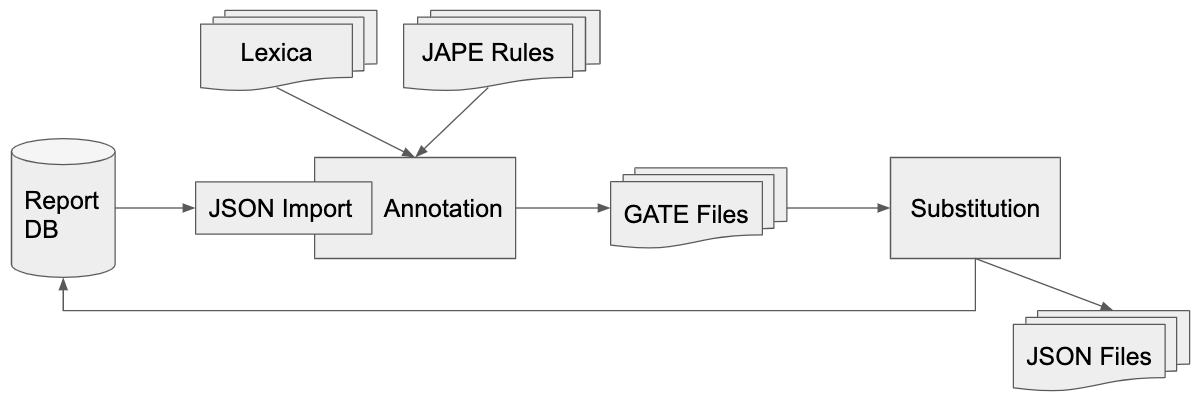
\includegraphics[width=\textwidth]{figs/system_overview.png}
\caption{System overview}
\end{figure}

\subsection{Document Import}\label{document-import}

The deidentifier tool imports JSON reports typically from a database
(json reports on the filesystem are also supported) and converts them to
a GATE compatible representation. The \texttt{annotate} command can read
directly from the appropriate source. The \texttt{import} command only
does the import and conversion step and stores a batch of documents into
a GATE corpus (which is a directory on a filesystem).

It is assumed that the documents are stored in a database table or view,
one row per document. The actual report content is encoded as JSON
string in one of the columns. Other required columns denote the document
type (\texttt{FCODE}) as well as the report id.

The tree like structure of the JSON documents is preserved during the
conversion to the GATE compatible representation. This can be exploited
during the annotation.

\subsection{annotate}\label{annotate}

The \texttt{annotate} command takes documents from a GATE corpus and
runs an annotation pipeline over the reports, i.e.~annotates portions of
the text which contain entities to be deidentified. The output of this
process is again a GATE corpus, which can be examined e.g.~using the
\href{https://gate.ac.uk/download/}{GATE developer tool}.

An \emph{annotation} simply denotes a span of text with some properties
associated, for example: ``Mr.~Muster, born 01.01.1964 in Aarau'' could
have 3 annotations related to deidentification: one for `Muster' (Name),
another for `01.01.1964' (Date, with the additional information that it
is a birthdate) and `Aarau' (Location).

Currently, the following entities are annotated: * Age * Contact
(distinguishing phone numbers, email and websites) * Date (if possible
determining birth date, admission date, discharge date) * ID (patient or
case ID, social security or insurance numbers) * Name (if possible
distinguishing patient from staff) * Location (broad category containing
geographical locations as well as organizations) * Occupation

The annotation pipeline consists basically of the following consecutive
steps:

\begin{figure}
\centering
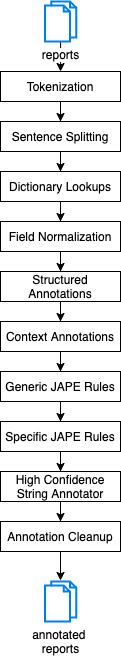
\includegraphics[width=0.2\textwidth]{figs/pipeline_overview.png}
\caption{Pipeline steps}
\end{figure}

\begin{enumerate}
\def\labelenumi{\arabic{enumi}.}
\tightlist
\item
  \textbf{Tokenization}: splitting the text into units of characters
  (`words'), for example `Mr.~Muster' would be split into 3 tokens `Mr',
  `.' and `Muster'
\item
  \textbf{Sentence Splitting}: Grouping tokens together into sentences
\item
  \textbf{Lookups}: Annotating tokens using dictionaries/lexica (called
  ``Gazetteers'' in GATE). For instance, the tokens `Universitätsspital
  Zürich' could be annotated as ``organsation'' and the token ``Zürich''
  as ``location''
\item
  \textbf{Field Normalization}: Renaming some fields in the report to a
  common name to simplify downstream steps. E.g. \texttt{AddrLine},
  \texttt{Address}, \texttt{Adresse} could all be renamed to
  \texttt{AddressField}.
\item
  \textbf{Structured Annotation}: annotate entire fields known to
  contain information to be deidentified. For example, the content of a
  field \texttt{Tel} denoting a phone number could immediately be
  annotated without having to apply any further processing.
\item
  \textbf{Context Annotation}: annotate a window (of tokens) around some
  trigger token with a \href{components.md\#context-annotations}{context
  annotation}. like \texttt{NameContext} or \texttt{OccupationContext}
  to help JAPE rules to disambiguate between e.g.~surnames and
  professions.
\item
  \textbf{JAPE rules}: annotate tokens based on a regular
  expression-like language. This is based on the structure or content of
  tokens (e.g.~a specific trigger word such as ``Dr'' or being a number)
  as well as previous annotations from dictionaries from the previous
  step. Note, that rules can also exploit the tree-like structure of the
  document, for example a rule may only apply if the token in a field is
  part of the section of the document related to patient information.
\item
  \textbf{High Confidence String Annotator}: Some JAPE rules in the
  previous step can be marked as \texttt{high\ confidence}, that is,
  whatever these rules annotate, we have high confidence that it is
  correct. The \texttt{HighConfidenceStringAnnotator} then checks what
  tokens were annotated by a high confidence rule and then annotates the
  same tokens in the remaining document.
\item
  \textbf{Clean up}: resolve overlapping or conflicting annotations
  using heuristics.
\end{enumerate}

\subsubsection{JAPE Example}\label{jape-example}

Here an example of a JAPE rule. We are interested in recognizing ages in
a very specific pattern, namely the age followed by ``jährige'',
``jähriger'' or ``jährigen'', e.g.~``59-jähriger Patient'':

\begin{verbatim}
// 0-119 (including decimals)
Macro: POSSIBLE_AGE
(
    ({Token.string ==~ "[1-9]*[0-9]"} | {Token.string ==~ "1[0-1][0-9]"})
    ({Token.string == "."} {Token.string ==~ "[0-9]+"})?
)


Rule: AgeRightContextTrigger
(
   (POSSIBLE_AGE):age
   ({Token.string == "-"})?
   ({Token.string ==~ "jährige[rn]?"})
)
-->
:age.Age = {rule = "AgeRightContextTrigger"}
\end{verbatim}

Rules describe a sequence of tokens on the ``left hand side'',
i.e.~before ``--\textgreater{}''. If such a sequence is recognized in a
text a rule is triggered and the ``right hand side'' is applied. In the
above case, the right hand side adds an annotation of type \texttt{Age}
having as a property the name of the rule triggered (this helps
debugging).

A token can be described exactly, like
\texttt{\{Token.string\ ==\ "-"\}} where the token should consist
exactly of \texttt{-} or using regular expressions as in
\texttt{\{Token.string\ ==\textasciitilde{}\ "1{[}0-1{]}{[}0-9{]}"\}}
describing the numbers from 100 to 119. A sequence of tokens may contain
optional elements denoted with \texttt{?}. In the above example the
\texttt{(\{Token.string\ ==\ "-"\})?} signifies, that there may or may
not be a dash.

More details regarding JAPE can be found in the
\href{https://gate.ac.uk/sale/thakker-jape-tutorial/GATE\%20JAPE\%20manual.pdf}{JAPE
Grammar Tutorial}

Note, that the above example is not robust against typos, e.g.~the rule
would fail to annotate the age in ``59-järiger Patient''.

\subsection{substitute}\label{substitute}

Takes an annotated GATE corpus and generates a JSON representation of
the content with to be deidentified tokens replaced. The JSON version of
these reports can then be saved back to a database table or to JSON
files on a drive one per report.

\subsubsection{Substitution Policies}\label{substitution-policies}

There are several policies implemented on how annotated tokens should be
replaced:

\begin{itemize}
\tightlist
\item
  \texttt{ScrubberSubstitution}: entities are replaced by a fixed string
  depending on the annotation type, for example `am 01.02.2003' would be
  replaced as ``am DATE'' and `Dr.~Muster' by `Dr.~NAME'
\item
  \texttt{DateShift}: same as \texttt{ScrubberSubstitution}, but all
  dates of a report are shifted by a random amount of days into the
  future or past.
\item
  \texttt{ReplacementTags}: In this policy information are passed along
  to a downstream application which takes care of the actual
  deidentification. For that purpose entities are replaced by `tags'
  which contain as much information as possible from the annotation
  pipeline. For example a text like ``Dr.~P. Muster empfiehlt'' could be
  replaced by
  \texttt{Dr.\ {[}{[}{[}Name;P.\ Muster;firstname=P;lastname=Muster;type=medical\ staff{]}{]}{]}\ empfiehlt}
  that is, the original value is preserved and the downstream
  application can decide how to replace the name most appropriately.
\end{itemize}

There exist also the \texttt{-\/-fields-blacklist} option, where a list
of field names can be provided which are completely erased from the
document. This can be useful for fields with are notoriously hard to
deidentify, but contain no relevant information for a downstream
application.
